\documentclass[twoside]{book}

% Packages required by doxygen
\usepackage{calc}
\usepackage{doxygen}
\usepackage{graphicx}
\usepackage[utf8]{inputenc}
\usepackage{makeidx}
\usepackage{multicol}
\usepackage{multirow}
\usepackage{fixltx2e}
\PassOptionsToPackage{warn}{textcomp}
\usepackage{textcomp}
\usepackage[nointegrals]{wasysym}
\usepackage[table]{xcolor}

% Font selection
\usepackage[T1]{fontenc}
\usepackage{mathptmx}
\usepackage[scaled=.90]{helvet}
\usepackage{courier}
\usepackage{amssymb}
\usepackage{sectsty}
\renewcommand{\familydefault}{\sfdefault}
\allsectionsfont{%
  \fontseries{bc}\selectfont%
  \color{darkgray}%
}
\renewcommand{\DoxyLabelFont}{%
  \fontseries{bc}\selectfont%
  \color{darkgray}%
}
\newcommand{\+}{\discretionary{\mbox{\scriptsize$\hookleftarrow$}}{}{}}

% Page & text layout
\usepackage{geometry}
\geometry{%
  a4paper,%
  top=2.5cm,%
  bottom=2.5cm,%
  left=2.5cm,%
  right=2.5cm%
}
\tolerance=750
\hfuzz=15pt
\hbadness=750
\setlength{\emergencystretch}{15pt}
\setlength{\parindent}{0cm}
\setlength{\parskip}{0.2cm}
\makeatletter
\renewcommand{\paragraph}{%
  \@startsection{paragraph}{4}{0ex}{-1.0ex}{1.0ex}{%
    \normalfont\normalsize\bfseries\SS@parafont%
  }%
}
\renewcommand{\subparagraph}{%
  \@startsection{subparagraph}{5}{0ex}{-1.0ex}{1.0ex}{%
    \normalfont\normalsize\bfseries\SS@subparafont%
  }%
}
\makeatother

% Headers & footers
\usepackage{fancyhdr}
\pagestyle{fancyplain}
\fancyhead[LE]{\fancyplain{}{\bfseries\thepage}}
\fancyhead[CE]{\fancyplain{}{}}
\fancyhead[RE]{\fancyplain{}{\bfseries\leftmark}}
\fancyhead[LO]{\fancyplain{}{\bfseries\rightmark}}
\fancyhead[CO]{\fancyplain{}{}}
\fancyhead[RO]{\fancyplain{}{\bfseries\thepage}}
\fancyfoot[LE]{\fancyplain{}{}}
\fancyfoot[CE]{\fancyplain{}{}}
\fancyfoot[RE]{\fancyplain{}{\bfseries\scriptsize Generated on Mon Dec 7 2015 17\+:02\+:13 for My Project by Doxygen }}
\fancyfoot[LO]{\fancyplain{}{\bfseries\scriptsize Generated on Mon Dec 7 2015 17\+:02\+:13 for My Project by Doxygen }}
\fancyfoot[CO]{\fancyplain{}{}}
\fancyfoot[RO]{\fancyplain{}{}}
\renewcommand{\footrulewidth}{0.4pt}
\renewcommand{\chaptermark}[1]{%
  \markboth{#1}{}%
}
\renewcommand{\sectionmark}[1]{%
  \markright{\thesection\ #1}%
}

% Indices & bibliography
\usepackage{natbib}
\usepackage[titles]{tocloft}
\setcounter{tocdepth}{3}
\setcounter{secnumdepth}{5}
\makeindex

% Hyperlinks (required, but should be loaded last)
\usepackage{ifpdf}
\ifpdf
  \usepackage[pdftex,pagebackref=true]{hyperref}
\else
  \usepackage[ps2pdf,pagebackref=true]{hyperref}
\fi
\hypersetup{%
  colorlinks=true,%
  linkcolor=blue,%
  citecolor=blue,%
  unicode%
}

% Custom commands
\newcommand{\clearemptydoublepage}{%
  \newpage{\pagestyle{empty}\cleardoublepage}%
}


%===== C O N T E N T S =====

\begin{document}

% Titlepage & ToC
\hypersetup{pageanchor=false,
             bookmarks=true,
             bookmarksnumbered=true,
             pdfencoding=unicode
            }
\pagenumbering{roman}
\begin{titlepage}
\vspace*{7cm}
\begin{center}%
{\Large My Project }\\
\vspace*{1cm}
{\large Generated by Doxygen 1.8.7}\\
\vspace*{0.5cm}
{\small Mon Dec 7 2015 17:02:13}\\
\end{center}
\end{titlepage}
\clearemptydoublepage
\tableofcontents
\clearemptydoublepage
\pagenumbering{arabic}
\hypersetup{pageanchor=true}

%--- Begin generated contents ---
\chapter{Hierarchical Index}
\section{Class Hierarchy}
This inheritance list is sorted roughly, but not completely, alphabetically\+:\begin{DoxyCompactList}
\item \contentsline{section}{mystl\+:\+:graph$<$ Vertex\+Property, Edge\+Property $>$}{\pageref{classmystl_1_1graph}}{}
\item \contentsline{section}{mystl\+:\+:graph$<$ Vertex\+Property, Edge\+Property $>$\+:\+:M\+S\+T\+Compare}{\pageref{classmystl_1_1graph_1_1MSTCompare}}{}
\item \contentsline{section}{mystl\+:\+:graph$<$ Vertex\+Property, Edge\+Property $>$\+:\+:M\+S\+T\+Label}{\pageref{classmystl_1_1graph_1_1MSTLabel}}{}
\item \contentsline{section}{test\+\_\+class}{\pageref{classtest__class}}{}
\begin{DoxyCompactList}
\item \contentsline{section}{graph\+\_\+test}{\pageref{classgraph__test}}{}
\end{DoxyCompactList}
\end{DoxyCompactList}

\chapter{Class Index}
\section{Class List}
Here are the classes, structs, unions and interfaces with brief descriptions\+:\begin{DoxyCompactList}
\item\contentsline{section}{\hyperlink{classmystl_1_1graph}{mystl\+::graph$<$ Vertex\+Property, Edge\+Property $>$} \\*Graph A\+D\+T based on C++ map implemented with two sets }{\pageref{classmystl_1_1graph}}{}
\item\contentsline{section}{\hyperlink{classgraph__test}{graph\+\_\+test} \\*Testing of graph \begin{DoxyVerb}\end{DoxyVerb}
 }{\pageref{classgraph__test}}{}
\item\contentsline{section}{\hyperlink{classmystl_1_1graph_1_1MSTCompare}{mystl\+::graph$<$ Vertex\+Property, Edge\+Property $>$\+::\+M\+S\+T\+Compare} \\*Compare class used by M\+S\+T\+\_\+prim\+\_\+jarniks compares distance from cloud of two vertex iterators }{\pageref{classmystl_1_1graph_1_1MSTCompare}}{}
\item\contentsline{section}{\hyperlink{classmystl_1_1graph_1_1MSTLabel}{mystl\+::graph$<$ Vertex\+Property, Edge\+Property $>$\+::\+M\+S\+T\+Label} \\*Label class used by M\+S\+T\+\_\+prim\+\_\+jarniks stores a distance and vertex descriptor for the parent }{\pageref{classmystl_1_1graph_1_1MSTLabel}}{}
\item\contentsline{section}{\hyperlink{classtest__class}{test\+\_\+class} \\*Test class for unit test framework \begin{DoxyVerb}\end{DoxyVerb}
 }{\pageref{classtest__class}}{}
\end{DoxyCompactList}

\chapter{Class Documentation}
\hypertarget{classmystl_1_1graph}{\section{mystl\+:\+:graph$<$ Vertex\+Property, Edge\+Property $>$ Class Template Reference}
\label{classmystl_1_1graph}\index{mystl\+::graph$<$ Vertex\+Property, Edge\+Property $>$@{mystl\+::graph$<$ Vertex\+Property, Edge\+Property $>$}}
}


Graph A\+D\+T based on C++ map implemented with two sets.  




{\ttfamily \#include $<$graph.\+h$>$}

\subsection*{Classes}
\begin{DoxyCompactItemize}
\item 
class \hyperlink{classmystl_1_1graph_1_1MSTCompare}{M\+S\+T\+Compare}
\begin{DoxyCompactList}\small\item\em Compare class used by M\+S\+T\+\_\+prim\+\_\+jarniks compares distance from cloud of two vertex iterators. \end{DoxyCompactList}\item 
class \hyperlink{classmystl_1_1graph_1_1MSTLabel}{M\+S\+T\+Label}
\begin{DoxyCompactList}\small\item\em Label class used by M\+S\+T\+\_\+prim\+\_\+jarniks stores a distance and vertex descriptor for the parent. \end{DoxyCompactList}\end{DoxyCompactItemize}
\subsection*{Public Types}
\begin{DoxyCompactItemize}
\item 
\hypertarget{classmystl_1_1graph_ad2732d0343911bde1277a7b8b293c256}{typedef size\+\_\+t \hyperlink{classmystl_1_1graph_ad2732d0343911bde1277a7b8b293c256}{vertex\+\_\+descriptor}}\label{classmystl_1_1graph_ad2732d0343911bde1277a7b8b293c256}

\begin{DoxyCompactList}\small\item\em required public types \end{DoxyCompactList}\item 
\hypertarget{classmystl_1_1graph_a36553c01984bf2cbdce92f6da743ca51}{typedef pair$<$ size\+\_\+t, size\+\_\+t $>$ {\bfseries edge\+\_\+descriptor}}\label{classmystl_1_1graph_a36553c01984bf2cbdce92f6da743ca51}

\item 
\hypertarget{classmystl_1_1graph_a2b72433f37e8f49ea4eb33237aaf7840}{typedef set$<$ shared\+\_\+ptr\\*
$<$ vertex $>$ $>$\+::iterator {\bfseries vertex\+\_\+iterator}}\label{classmystl_1_1graph_a2b72433f37e8f49ea4eb33237aaf7840}

\item 
\hypertarget{classmystl_1_1graph_a62aba2cfdc9b8487be4016c71088c11e}{typedef set$<$ shared\+\_\+ptr\\*
$<$ vertex $>$ $>$\+::const\+\_\+iterator {\bfseries const\+\_\+vertex\+\_\+iterator}}\label{classmystl_1_1graph_a62aba2cfdc9b8487be4016c71088c11e}

\item 
\hypertarget{classmystl_1_1graph_ae516cab08fa293faf4c126487932759a}{typedef set$<$ shared\+\_\+ptr$<$ edge $>$\\*
 $>$\+::iterator {\bfseries edge\+\_\+iterator}}\label{classmystl_1_1graph_ae516cab08fa293faf4c126487932759a}

\item 
\hypertarget{classmystl_1_1graph_a1479778e9a47b879c7c77c4e6ab63cd6}{typedef set$<$ shared\+\_\+ptr$<$ edge $>$\\*
 $>$\+::const\+\_\+iterator {\bfseries const\+\_\+edge\+\_\+iterator}}\label{classmystl_1_1graph_a1479778e9a47b879c7c77c4e6ab63cd6}

\item 
\hypertarget{classmystl_1_1graph_ac74fa1c083b1041103a20544fcbf7c17}{typedef set$<$ shared\+\_\+ptr$<$ edge $>$\\*
 $>$\+::iterator {\bfseries adj\+\_\+edge\+\_\+iterator}}\label{classmystl_1_1graph_ac74fa1c083b1041103a20544fcbf7c17}

\item 
\hypertarget{classmystl_1_1graph_a01df49c28ef2f886d600175055cd2915}{typedef set$<$ shared\+\_\+ptr$<$ edge $>$\\*
 $>$\+::const\+\_\+iterator {\bfseries const\+\_\+adj\+\_\+edge\+\_\+iterator}}\label{classmystl_1_1graph_a01df49c28ef2f886d600175055cd2915}

\end{DoxyCompactItemize}
\begin{Indent}{\bf Types}\par
{\em Forward declared edge\+\_\+comp comparator class

required public types }\begin{DoxyCompactItemize}
\item 
\hypertarget{classmystl_1_1graph_ae8d072039125c2536419b9d4ad1ca577}{enum {\bfseries Label} \{ \\*
{\bfseries V\+I\+S\+I\+T\+E\+D} =0, 
{\bfseries U\+N\+V\+I\+S\+I\+T\+E\+D}, 
{\bfseries D\+I\+S\+C\+O\+V\+E\+R\+E\+D}, 
{\bfseries C\+R\+O\+S\+S}, 
\\*
{\bfseries B\+A\+C\+K}
 \}}\label{classmystl_1_1graph_ae8d072039125c2536419b9d4ad1ca577}

\item 
\hypertarget{classmystl_1_1graph_ad2732d0343911bde1277a7b8b293c256}{typedef size\+\_\+t {\bfseries vertex\+\_\+descriptor}}\label{classmystl_1_1graph_ad2732d0343911bde1277a7b8b293c256}

\item 
\hypertarget{classmystl_1_1graph_a5e841bf3fc28d6cec2de2ea326cd83ea}{typedef std\+::pair$<$ size\+\_\+t, size\+\_\+t $>$ {\bfseries edge\+\_\+descriptor}}\label{classmystl_1_1graph_a5e841bf3fc28d6cec2de2ea326cd83ea}

\item 
\hypertarget{classmystl_1_1graph_a173b6e21e17fd9bafdd7594b2ba3ef0a}{typedef std\+::set$<$ vertex $\ast$ $>$\\*
\+::iterator \hyperlink{classmystl_1_1graph_a173b6e21e17fd9bafdd7594b2ba3ef0a}{vertex\+\_\+iterator}}\label{classmystl_1_1graph_a173b6e21e17fd9bafdd7594b2ba3ef0a}

\begin{DoxyCompactList}\small\item\em vertex iterators \end{DoxyCompactList}\item 
\hypertarget{classmystl_1_1graph_a4b4067e095744d85290e63cb4c7c6d53}{typedef std\+::set$<$ vertex $\ast$ $>$\\*
\+::const\+\_\+iterator {\bfseries const\+\_\+vertex\+\_\+iterator}}\label{classmystl_1_1graph_a4b4067e095744d85290e63cb4c7c6d53}

\item 
\hypertarget{classmystl_1_1graph_aca4e86526b9606bc4a568b0c4e127b3f}{typedef std\+::set$<$ edge $\ast$ $>$\\*
\+::iterator \hyperlink{classmystl_1_1graph_aca4e86526b9606bc4a568b0c4e127b3f}{edge\+\_\+iterator}}\label{classmystl_1_1graph_aca4e86526b9606bc4a568b0c4e127b3f}

\begin{DoxyCompactList}\small\item\em edge iterators \end{DoxyCompactList}\item 
\hypertarget{classmystl_1_1graph_af3f7ff404779108f31fccec55a84cae2}{typedef std\+::set$<$ edge $\ast$ $>$\\*
\+::const\+\_\+iterator {\bfseries const\+\_\+edge\+\_\+iterator}}\label{classmystl_1_1graph_af3f7ff404779108f31fccec55a84cae2}

\item 
\hypertarget{classmystl_1_1graph_a1eecb1e0d123a8bd3987658cd8da3adb}{typedef std\+::set$<$ edge $\ast$ $>$\\*
\+::iterator {\bfseries adj\+\_\+edge\+\_\+iterator}}\label{classmystl_1_1graph_a1eecb1e0d123a8bd3987658cd8da3adb}

\item 
\hypertarget{classmystl_1_1graph_a78fdafef556df27b9f0c92d87b20a9c1}{typedef std\+::set$<$ edge $\ast$ $>$\\*
\+::const\+\_\+iterator {\bfseries const\+\_\+adj\+\_\+edge\+\_\+iterator}}\label{classmystl_1_1graph_a78fdafef556df27b9f0c92d87b20a9c1}

\end{DoxyCompactItemize}
\end{Indent}
\subsection*{Public Member Functions}
\begin{DoxyCompactItemize}
\item 
size\+\_\+t \hyperlink{classmystl_1_1graph_aa6fd8efc0911be8bd65f659d4d717bc9}{num\+\_\+vertices} () const 
\item 
size\+\_\+t \hyperlink{classmystl_1_1graph_a659585bd8325746aa743b5103753405b}{num\+\_\+edges} () const 
\item 
\hypertarget{classmystl_1_1graph_ab7e28ce8dedb8b396c8912b6aacf263d}{void {\bfseries clear} ()}\label{classmystl_1_1graph_ab7e28ce8dedb8b396c8912b6aacf263d}

\item 
\hypertarget{classmystl_1_1graph_a3bd4b577259268bb5ddc09953d5bbdd4}{\hyperlink{classmystl_1_1graph_a3bd4b577259268bb5ddc09953d5bbdd4}{graph} ()}\label{classmystl_1_1graph_a3bd4b577259268bb5ddc09953d5bbdd4}

\begin{DoxyCompactList}\small\item\em required constructor/destructors \end{DoxyCompactList}\item 
\hypertarget{classmystl_1_1graph_aaaec7844368eb2450398bd41c313a464}{{\bfseries graph} (const \hyperlink{classmystl_1_1graph}{graph} \&)=delete}\label{classmystl_1_1graph_aaaec7844368eb2450398bd41c313a464}

\item 
\hypertarget{classmystl_1_1graph_a331b19cbe43fab284d3329962dc2d15b}{\hyperlink{classmystl_1_1graph}{graph} \& {\bfseries operator=} (const \hyperlink{classmystl_1_1graph}{graph} \&)=delete}\label{classmystl_1_1graph_a331b19cbe43fab284d3329962dc2d15b}

\item 
\hypertarget{classmystl_1_1graph_af345ac781b3c5f8c5507b26750e80db5}{\hyperlink{classmystl_1_1graph_a173b6e21e17fd9bafdd7594b2ba3ef0a}{vertex\+\_\+iterator} \hyperlink{classmystl_1_1graph_af345ac781b3c5f8c5507b26750e80db5}{vertices\+\_\+begin} ()}\label{classmystl_1_1graph_af345ac781b3c5f8c5507b26750e80db5}

\begin{DoxyCompactList}\small\item\em required graph operations \end{DoxyCompactList}\item 
\hypertarget{classmystl_1_1graph_a7132eb9c3130efa49e521ff5d64de659}{const\+\_\+vertex\+\_\+iterator {\bfseries vertices\+\_\+cbegin} () const }\label{classmystl_1_1graph_a7132eb9c3130efa49e521ff5d64de659}

\item 
\hypertarget{classmystl_1_1graph_ae03d839b0bc65ae3337519aa791ac485}{\hyperlink{classmystl_1_1graph_a173b6e21e17fd9bafdd7594b2ba3ef0a}{vertex\+\_\+iterator} {\bfseries vertices\+\_\+end} ()}\label{classmystl_1_1graph_ae03d839b0bc65ae3337519aa791ac485}

\item 
\hypertarget{classmystl_1_1graph_ae6dc5a4a8da0990502bfcd146854a305}{const\+\_\+vertex\+\_\+iterator {\bfseries vertices\+\_\+cend} () const }\label{classmystl_1_1graph_ae6dc5a4a8da0990502bfcd146854a305}

\item 
\hypertarget{classmystl_1_1graph_af61b17c57aeb83bf8c66979276ad7941}{\hyperlink{classmystl_1_1graph_aca4e86526b9606bc4a568b0c4e127b3f}{edge\+\_\+iterator} {\bfseries edges\+\_\+begin} ()}\label{classmystl_1_1graph_af61b17c57aeb83bf8c66979276ad7941}

\item 
\hypertarget{classmystl_1_1graph_ace540bc4fda9c0a5a6701c252af21a1a}{const\+\_\+edge\+\_\+iterator {\bfseries edges\+\_\+cbegin} () const }\label{classmystl_1_1graph_ace540bc4fda9c0a5a6701c252af21a1a}

\item 
\hypertarget{classmystl_1_1graph_aecd73d2b1bebbe9ea30f813709db1006}{\hyperlink{classmystl_1_1graph_aca4e86526b9606bc4a568b0c4e127b3f}{edge\+\_\+iterator} {\bfseries edges\+\_\+end} ()}\label{classmystl_1_1graph_aecd73d2b1bebbe9ea30f813709db1006}

\item 
\hypertarget{classmystl_1_1graph_adfecdeafcf7092e0f715ebd9c221c1bd}{const\+\_\+edge\+\_\+iterator {\bfseries edges\+\_\+cend} () const }\label{classmystl_1_1graph_adfecdeafcf7092e0f715ebd9c221c1bd}

\item 
\hypertarget{classmystl_1_1graph_aa6fd8efc0911be8bd65f659d4d717bc9}{size\+\_\+t {\bfseries num\+\_\+vertices} () const }\label{classmystl_1_1graph_aa6fd8efc0911be8bd65f659d4d717bc9}

\item 
\hypertarget{classmystl_1_1graph_a659585bd8325746aa743b5103753405b}{size\+\_\+t {\bfseries num\+\_\+edges} () const }\label{classmystl_1_1graph_a659585bd8325746aa743b5103753405b}

\item 
\hypertarget{classmystl_1_1graph_a1565ecbd61037a48bee3e0d969c6b57b}{\hyperlink{classmystl_1_1graph_a173b6e21e17fd9bafdd7594b2ba3ef0a}{vertex\+\_\+iterator} {\bfseries find\+\_\+vertex} (vertex\+\_\+descriptor v\+\_\+descriptor)}\label{classmystl_1_1graph_a1565ecbd61037a48bee3e0d969c6b57b}

\item 
\hypertarget{classmystl_1_1graph_a7870e4532e14ceadfd59838e6c4dcd0c}{const\+\_\+vertex\+\_\+iterator {\bfseries find\+\_\+vertex} (vertex\+\_\+descriptor v\+\_\+descriptor) const }\label{classmystl_1_1graph_a7870e4532e14ceadfd59838e6c4dcd0c}

\item 
\hypertarget{classmystl_1_1graph_ab62c660d618a35dd79ad7d2e5296a6c6}{\hyperlink{classmystl_1_1graph_aca4e86526b9606bc4a568b0c4e127b3f}{edge\+\_\+iterator} {\bfseries find\+\_\+edge} (edge\+\_\+descriptor e\+\_\+descriptor)}\label{classmystl_1_1graph_ab62c660d618a35dd79ad7d2e5296a6c6}

\item 
\hypertarget{classmystl_1_1graph_ab248f0d7d62bd50d6a80746d3cf63fb1}{const\+\_\+edge\+\_\+iterator {\bfseries find\+\_\+edge} (edge\+\_\+descriptor e\+\_\+descriptor) const }\label{classmystl_1_1graph_ab248f0d7d62bd50d6a80746d3cf63fb1}

\item 
\hypertarget{classmystl_1_1graph_a113159cdbf74506664abc3a80c317965}{vertex\+\_\+descriptor {\bfseries insert\+\_\+vertex} (const Vertex\+Property \&property)}\label{classmystl_1_1graph_a113159cdbf74506664abc3a80c317965}

\item 
\hypertarget{classmystl_1_1graph_aa4dfab685cad6afd7e8844dce5677503}{edge\+\_\+descriptor {\bfseries insert\+\_\+edge} (vertex\+\_\+descriptor v\+\_\+src, vertex\+\_\+descriptor v\+\_\+dest, const Edge\+Property \&property)}\label{classmystl_1_1graph_aa4dfab685cad6afd7e8844dce5677503}

\item 
\hypertarget{classmystl_1_1graph_a4d25045a4836e8f45e96963825a5473e}{void {\bfseries insert\+\_\+edge\+\_\+undirected} (vertex\+\_\+descriptor v\+\_\+src, vertex\+\_\+descriptor v\+\_\+dest, const Edge\+Property \&property)}\label{classmystl_1_1graph_a4d25045a4836e8f45e96963825a5473e}

\item 
\hypertarget{classmystl_1_1graph_a744d4aadf26398d64c4a162e8a5a47b0}{void {\bfseries erase\+\_\+vertex} (vertex\+\_\+descriptor v\+\_\+descriptor)}\label{classmystl_1_1graph_a744d4aadf26398d64c4a162e8a5a47b0}

\item 
\hypertarget{classmystl_1_1graph_a476bcdd8e98edf1f53db62a20f50747e}{void {\bfseries erase\+\_\+edge} (edge\+\_\+descriptor e\+\_\+descriptor)}\label{classmystl_1_1graph_a476bcdd8e98edf1f53db62a20f50747e}

\item 
\hypertarget{classmystl_1_1graph_ab7e28ce8dedb8b396c8912b6aacf263d}{void {\bfseries clear} ()}\label{classmystl_1_1graph_ab7e28ce8dedb8b396c8912b6aacf263d}

\end{DoxyCompactItemize}
\begin{Indent}{\bf Constructors}\par
{\em required constructor/destructors }\begin{DoxyCompactItemize}
\item 
\hypertarget{classmystl_1_1graph_a3bd4b577259268bb5ddc09953d5bbdd4}{\hyperlink{classmystl_1_1graph_a3bd4b577259268bb5ddc09953d5bbdd4}{graph} ()}\label{classmystl_1_1graph_a3bd4b577259268bb5ddc09953d5bbdd4}

\begin{DoxyCompactList}\small\item\em Constructor. \end{DoxyCompactList}\item 
\hypertarget{classmystl_1_1graph_a18df46cc1311ba1999f0ce3cdf1ab21c}{\hyperlink{classmystl_1_1graph_a18df46cc1311ba1999f0ce3cdf1ab21c}{$\sim$graph} ()}\label{classmystl_1_1graph_a18df46cc1311ba1999f0ce3cdf1ab21c}

\begin{DoxyCompactList}\small\item\em Destructor. \end{DoxyCompactList}\item 
\hypertarget{classmystl_1_1graph_aaaec7844368eb2450398bd41c313a464}{\hyperlink{classmystl_1_1graph_aaaec7844368eb2450398bd41c313a464}{graph} (const \hyperlink{classmystl_1_1graph}{graph} \&)=delete}\label{classmystl_1_1graph_aaaec7844368eb2450398bd41c313a464}

\begin{DoxyCompactList}\small\item\em Copy Constructor. \end{DoxyCompactList}\item 
\hypertarget{classmystl_1_1graph_a331b19cbe43fab284d3329962dc2d15b}{\hyperlink{classmystl_1_1graph}{graph} \& \hyperlink{classmystl_1_1graph_a331b19cbe43fab284d3329962dc2d15b}{operator=} (const \hyperlink{classmystl_1_1graph}{graph} \&)=delete}\label{classmystl_1_1graph_a331b19cbe43fab284d3329962dc2d15b}

\begin{DoxyCompactList}\small\item\em Assignment operator. \end{DoxyCompactList}\end{DoxyCompactItemize}
\end{Indent}
\begin{Indent}{\bf Iterators}\par
{\em required graph operations }\begin{DoxyCompactItemize}
\item 
\hypertarget{classmystl_1_1graph_af345ac781b3c5f8c5507b26750e80db5}{\hyperlink{classmystl_1_1graph_a173b6e21e17fd9bafdd7594b2ba3ef0a}{vertex\+\_\+iterator} {\bfseries vertices\+\_\+begin} ()}\label{classmystl_1_1graph_af345ac781b3c5f8c5507b26750e80db5}

\item 
\hypertarget{classmystl_1_1graph_a7132eb9c3130efa49e521ff5d64de659}{const\+\_\+vertex\+\_\+iterator {\bfseries vertices\+\_\+cbegin} () const }\label{classmystl_1_1graph_a7132eb9c3130efa49e521ff5d64de659}

\item 
\hypertarget{classmystl_1_1graph_ae03d839b0bc65ae3337519aa791ac485}{\hyperlink{classmystl_1_1graph_a173b6e21e17fd9bafdd7594b2ba3ef0a}{vertex\+\_\+iterator} {\bfseries vertices\+\_\+end} ()}\label{classmystl_1_1graph_ae03d839b0bc65ae3337519aa791ac485}

\item 
\hypertarget{classmystl_1_1graph_ae6dc5a4a8da0990502bfcd146854a305}{const\+\_\+vertex\+\_\+iterator {\bfseries vertices\+\_\+cend} () const }\label{classmystl_1_1graph_ae6dc5a4a8da0990502bfcd146854a305}

\item 
\hypertarget{classmystl_1_1graph_af61b17c57aeb83bf8c66979276ad7941}{\hyperlink{classmystl_1_1graph_aca4e86526b9606bc4a568b0c4e127b3f}{edge\+\_\+iterator} {\bfseries edges\+\_\+begin} ()}\label{classmystl_1_1graph_af61b17c57aeb83bf8c66979276ad7941}

\item 
\hypertarget{classmystl_1_1graph_ace540bc4fda9c0a5a6701c252af21a1a}{const\+\_\+edge\+\_\+iterator {\bfseries edges\+\_\+cbegin} () const }\label{classmystl_1_1graph_ace540bc4fda9c0a5a6701c252af21a1a}

\item 
\hypertarget{classmystl_1_1graph_aecd73d2b1bebbe9ea30f813709db1006}{\hyperlink{classmystl_1_1graph_aca4e86526b9606bc4a568b0c4e127b3f}{edge\+\_\+iterator} {\bfseries edges\+\_\+end} ()}\label{classmystl_1_1graph_aecd73d2b1bebbe9ea30f813709db1006}

\item 
\hypertarget{classmystl_1_1graph_adfecdeafcf7092e0f715ebd9c221c1bd}{const\+\_\+edge\+\_\+iterator {\bfseries edges\+\_\+cend} () const }\label{classmystl_1_1graph_adfecdeafcf7092e0f715ebd9c221c1bd}

\end{DoxyCompactItemize}
\end{Indent}
\begin{Indent}{\bf Entity Location}\par
\begin{DoxyCompactItemize}
\item 
\hyperlink{classmystl_1_1graph_a173b6e21e17fd9bafdd7594b2ba3ef0a}{vertex\+\_\+iterator} \hyperlink{classmystl_1_1graph_a9f9e02fc5c47418c60e60283aad779fa}{find\+\_\+vertex} (vertex\+\_\+descriptor vd)
\item 
const\+\_\+vertex\+\_\+iterator \hyperlink{classmystl_1_1graph_af0c7dfb55a41898adb8523b0fb95e9d9}{find\+\_\+vertex} (vertex\+\_\+descriptor vd) const 
\item 
\hyperlink{classmystl_1_1graph_aca4e86526b9606bc4a568b0c4e127b3f}{edge\+\_\+iterator} \hyperlink{classmystl_1_1graph_a6b9303727279b373f93a7a7b2117601b}{find\+\_\+edge} (edge\+\_\+descriptor ed)
\item 
const\+\_\+edge\+\_\+iterator \hyperlink{classmystl_1_1graph_a63796b6ea4e3dd28ce7e690257a90ffc}{find\+\_\+edge} (edge\+\_\+descriptor ed) const 
\end{DoxyCompactItemize}
\end{Indent}
\begin{Indent}{\bf Modifiers}\par
\begin{DoxyCompactItemize}
\item 
vertex\+\_\+descriptor \hyperlink{classmystl_1_1graph_a733a0df9553be6158ac4c4bbcb21fcea}{insert\+\_\+vertex} (const Vertex\+Property \&v)
\begin{DoxyCompactList}\small\item\em Insert a vertex into the graph with value v. \end{DoxyCompactList}\item 
edge\+\_\+descriptor \hyperlink{classmystl_1_1graph_ae4eee46747666daab648d8ffabb4fbbb}{insert\+\_\+edge} (const vertex\+\_\+descriptor vd1, const vertex\+\_\+descriptor vd2, const Edge\+Property \&e)
\begin{DoxyCompactList}\small\item\em Insert an edge into the graph with weight e. \end{DoxyCompactList}\item 
void \hyperlink{classmystl_1_1graph_a76f7a736aadd6c49c0a24eba2c8657ee}{insert\+\_\+edge\+\_\+undirected} (const vertex\+\_\+descriptor vd1, const vertex\+\_\+descriptor vd2, const Edge\+Property \&e)
\begin{DoxyCompactList}\small\item\em Insert an undirected edge into the graph with weight e. \end{DoxyCompactList}\item 
void \hyperlink{classmystl_1_1graph_acddd1e68646f4deb6b3d0bc90071a120}{erase\+\_\+vertex} (const vertex\+\_\+descriptor vd)
\begin{DoxyCompactList}\small\item\em erases a vertex from the graph \end{DoxyCompactList}\item 
void \hyperlink{classmystl_1_1graph_a9f54888f6de02668996fd9f5ec25769f}{erase\+\_\+edge} (const edge\+\_\+descriptor ed)
\begin{DoxyCompactList}\small\item\em Erase an edge from the graph. \end{DoxyCompactList}\end{DoxyCompactItemize}
\end{Indent}
\subsection*{Friends}
\begin{DoxyCompactItemize}
\item 
{\footnotesize template$<$typename V , typename E $>$ }\\std\+::istream \& \hyperlink{classmystl_1_1graph_aa5e68654c5943df7ebbc1bd6e9312121}{operator$>$$>$} (std\+::istream \&is, \hyperlink{classmystl_1_1graph}{graph}$<$ V, E $>$ \&g)
\begin{DoxyCompactList}\small\item\em input operator \end{DoxyCompactList}\item 
{\footnotesize template$<$typename V , typename E $>$ }\\std\+::ostream \& \hyperlink{classmystl_1_1graph_a9d5de7fa26f6baa171baa2700f707061}{operator$<$$<$} (std\+::ostream \&os, const \hyperlink{classmystl_1_1graph}{graph}$<$ V, E $>$ \&g)
\begin{DoxyCompactList}\small\item\em output operator \end{DoxyCompactList}\item 
\hypertarget{classmystl_1_1graph_a704c337be3ef404f576c510e45b3b150}{{\footnotesize template$<$typename V , typename E $>$ }\\istream \& {\bfseries operator$>$$>$} (istream \&in, \hyperlink{classmystl_1_1graph}{graph}$<$ V, E $>$ \&g)}\label{classmystl_1_1graph_a704c337be3ef404f576c510e45b3b150}

\item 
\hypertarget{classmystl_1_1graph_a2887971cf454be5bc66778aff744406d}{{\footnotesize template$<$typename V , typename E $>$ }\\ostream \& {\bfseries operator$<$$<$} (ostream \&out, const \hyperlink{classmystl_1_1graph}{graph}$<$ V, E $>$ \&g)}\label{classmystl_1_1graph_a2887971cf454be5bc66778aff744406d}

\end{DoxyCompactItemize}


\subsection{Detailed Description}
\subsubsection*{template$<$typename Vertex\+Property, typename Edge\+Property$>$class mystl\+::graph$<$ Vertex\+Property, Edge\+Property $>$}

Graph A\+D\+T based on C++ map implemented with two sets. 


\begin{DoxyTemplParams}{Template Parameters}
{\em Vertex\+Property} & vertex value type \\
\hline
{\em Edge\+Property} & edge weight type \\
\hline
\end{DoxyTemplParams}


\subsection{Member Function Documentation}
\hypertarget{classmystl_1_1graph_a9f54888f6de02668996fd9f5ec25769f}{\index{mystl\+::graph@{mystl\+::graph}!erase\+\_\+edge@{erase\+\_\+edge}}
\index{erase\+\_\+edge@{erase\+\_\+edge}!mystl\+::graph@{mystl\+::graph}}
\subsubsection[{erase\+\_\+edge}]{\setlength{\rightskip}{0pt plus 5cm}template$<$typename Vertex\+Property, typename Edge\+Property$>$ void {\bf mystl\+::graph}$<$ Vertex\+Property, Edge\+Property $>$\+::erase\+\_\+edge (
\begin{DoxyParamCaption}
\item[{const edge\+\_\+descriptor}]{ed}
\end{DoxyParamCaption}
)\hspace{0.3cm}{\ttfamily [inline]}}}\label{classmystl_1_1graph_a9f54888f6de02668996fd9f5ec25769f}


Erase an edge from the graph. 


\begin{DoxyParams}{Parameters}
{\em ed} & edge descriptor of the edge begin erased\\
\hline
\end{DoxyParams}
removes the edge from both target and source adjacency edge set \hypertarget{classmystl_1_1graph_acddd1e68646f4deb6b3d0bc90071a120}{\index{mystl\+::graph@{mystl\+::graph}!erase\+\_\+vertex@{erase\+\_\+vertex}}
\index{erase\+\_\+vertex@{erase\+\_\+vertex}!mystl\+::graph@{mystl\+::graph}}
\subsubsection[{erase\+\_\+vertex}]{\setlength{\rightskip}{0pt plus 5cm}template$<$typename Vertex\+Property, typename Edge\+Property$>$ void {\bf mystl\+::graph}$<$ Vertex\+Property, Edge\+Property $>$\+::erase\+\_\+vertex (
\begin{DoxyParamCaption}
\item[{const vertex\+\_\+descriptor}]{vd}
\end{DoxyParamCaption}
)\hspace{0.3cm}{\ttfamily [inline]}}}\label{classmystl_1_1graph_acddd1e68646f4deb6b3d0bc90071a120}


erases a vertex from the graph 


\begin{DoxyParams}{Parameters}
{\em vd} & vertex descriptor of vertex being erased\\
\hline
\end{DoxyParams}
erases any edge that is going to and from the vertex it must erase the edges in an opposite vertex's adjacent edge set \hypertarget{classmystl_1_1graph_a6b9303727279b373f93a7a7b2117601b}{\index{mystl\+::graph@{mystl\+::graph}!find\+\_\+edge@{find\+\_\+edge}}
\index{find\+\_\+edge@{find\+\_\+edge}!mystl\+::graph@{mystl\+::graph}}
\subsubsection[{find\+\_\+edge}]{\setlength{\rightskip}{0pt plus 5cm}template$<$typename Vertex\+Property, typename Edge\+Property$>$ {\bf edge\+\_\+iterator} {\bf mystl\+::graph}$<$ Vertex\+Property, Edge\+Property $>$\+::find\+\_\+edge (
\begin{DoxyParamCaption}
\item[{edge\+\_\+descriptor}]{ed}
\end{DoxyParamCaption}
)\hspace{0.3cm}{\ttfamily [inline]}}}\label{classmystl_1_1graph_a6b9303727279b373f93a7a7b2117601b}

\begin{DoxyParams}{Parameters}
{\em ed} & edge descriptor \\
\hline
\end{DoxyParams}
\begin{DoxyReturn}{Returns}
iterator to given edge descriptor
\end{DoxyReturn}
If {\ttfamily vd} matches any of the entities in the edge set then it return an iterator to the location in the sets

If {\ttfamily vd} is not found then an iterator to the end of the set will be returned \hypertarget{classmystl_1_1graph_a63796b6ea4e3dd28ce7e690257a90ffc}{\index{mystl\+::graph@{mystl\+::graph}!find\+\_\+edge@{find\+\_\+edge}}
\index{find\+\_\+edge@{find\+\_\+edge}!mystl\+::graph@{mystl\+::graph}}
\subsubsection[{find\+\_\+edge}]{\setlength{\rightskip}{0pt plus 5cm}template$<$typename Vertex\+Property, typename Edge\+Property$>$ const\+\_\+edge\+\_\+iterator {\bf mystl\+::graph}$<$ Vertex\+Property, Edge\+Property $>$\+::find\+\_\+edge (
\begin{DoxyParamCaption}
\item[{edge\+\_\+descriptor}]{ed}
\end{DoxyParamCaption}
) const\hspace{0.3cm}{\ttfamily [inline]}}}\label{classmystl_1_1graph_a63796b6ea4e3dd28ce7e690257a90ffc}

\begin{DoxyParams}{Parameters}
{\em ed} & edge descriptor \\
\hline
\end{DoxyParams}
\begin{DoxyReturn}{Returns}
iterator to given edge descriptor
\end{DoxyReturn}
If {\ttfamily vd} matches any of the entities in the edge set then it return an iterator to the location in the sets

If {\ttfamily vd} is not found then an iterator to the end of the set will be returned \hypertarget{classmystl_1_1graph_a9f9e02fc5c47418c60e60283aad779fa}{\index{mystl\+::graph@{mystl\+::graph}!find\+\_\+vertex@{find\+\_\+vertex}}
\index{find\+\_\+vertex@{find\+\_\+vertex}!mystl\+::graph@{mystl\+::graph}}
\subsubsection[{find\+\_\+vertex}]{\setlength{\rightskip}{0pt plus 5cm}template$<$typename Vertex\+Property, typename Edge\+Property$>$ {\bf vertex\+\_\+iterator} {\bf mystl\+::graph}$<$ Vertex\+Property, Edge\+Property $>$\+::find\+\_\+vertex (
\begin{DoxyParamCaption}
\item[{vertex\+\_\+descriptor}]{vd}
\end{DoxyParamCaption}
)\hspace{0.3cm}{\ttfamily [inline]}}}\label{classmystl_1_1graph_a9f9e02fc5c47418c60e60283aad779fa}

\begin{DoxyParams}{Parameters}
{\em vd} & vertex descriptor \\
\hline
\end{DoxyParams}
\begin{DoxyReturn}{Returns}
iterator to given vertex descriptor
\end{DoxyReturn}
If {\ttfamily vd} matches any of the entities in the vertex set then it return an iterator to the location in the sets

If {\ttfamily vd} is not found then an iterator to the end of the set will be returned \hypertarget{classmystl_1_1graph_af0c7dfb55a41898adb8523b0fb95e9d9}{\index{mystl\+::graph@{mystl\+::graph}!find\+\_\+vertex@{find\+\_\+vertex}}
\index{find\+\_\+vertex@{find\+\_\+vertex}!mystl\+::graph@{mystl\+::graph}}
\subsubsection[{find\+\_\+vertex}]{\setlength{\rightskip}{0pt plus 5cm}template$<$typename Vertex\+Property, typename Edge\+Property$>$ const\+\_\+vertex\+\_\+iterator {\bf mystl\+::graph}$<$ Vertex\+Property, Edge\+Property $>$\+::find\+\_\+vertex (
\begin{DoxyParamCaption}
\item[{vertex\+\_\+descriptor}]{vd}
\end{DoxyParamCaption}
) const\hspace{0.3cm}{\ttfamily [inline]}}}\label{classmystl_1_1graph_af0c7dfb55a41898adb8523b0fb95e9d9}

\begin{DoxyParams}{Parameters}
{\em vd} & vertex descriptor \\
\hline
\end{DoxyParams}
\begin{DoxyReturn}{Returns}
iterator to given vertex descriptor
\end{DoxyReturn}
If {\ttfamily vd} matches any of the entities in the vertex set then it return an iterator to the location in the sets

If {\ttfamily vd} is not found then an iterator to the end of the set will be returned \hypertarget{classmystl_1_1graph_ae4eee46747666daab648d8ffabb4fbbb}{\index{mystl\+::graph@{mystl\+::graph}!insert\+\_\+edge@{insert\+\_\+edge}}
\index{insert\+\_\+edge@{insert\+\_\+edge}!mystl\+::graph@{mystl\+::graph}}
\subsubsection[{insert\+\_\+edge}]{\setlength{\rightskip}{0pt plus 5cm}template$<$typename Vertex\+Property, typename Edge\+Property$>$ edge\+\_\+descriptor {\bf mystl\+::graph}$<$ Vertex\+Property, Edge\+Property $>$\+::insert\+\_\+edge (
\begin{DoxyParamCaption}
\item[{const vertex\+\_\+descriptor}]{vd1, }
\item[{const vertex\+\_\+descriptor}]{vd2, }
\item[{const Edge\+Property \&}]{e}
\end{DoxyParamCaption}
)\hspace{0.3cm}{\ttfamily [inline]}}}\label{classmystl_1_1graph_ae4eee46747666daab648d8ffabb4fbbb}


Insert an edge into the graph with weight e. 


\begin{DoxyParams}{Parameters}
{\em vd1} & vertex descriptor of the source vertex \\
\hline
{\em vd2} & vertex descriptor of the target vertex \\
\hline
\end{DoxyParams}
\begin{DoxyReturn}{Returns}
the edge descriptor the edge inserted 
\end{DoxyReturn}
\hypertarget{classmystl_1_1graph_a76f7a736aadd6c49c0a24eba2c8657ee}{\index{mystl\+::graph@{mystl\+::graph}!insert\+\_\+edge\+\_\+undirected@{insert\+\_\+edge\+\_\+undirected}}
\index{insert\+\_\+edge\+\_\+undirected@{insert\+\_\+edge\+\_\+undirected}!mystl\+::graph@{mystl\+::graph}}
\subsubsection[{insert\+\_\+edge\+\_\+undirected}]{\setlength{\rightskip}{0pt plus 5cm}template$<$typename Vertex\+Property, typename Edge\+Property$>$ void {\bf mystl\+::graph}$<$ Vertex\+Property, Edge\+Property $>$\+::insert\+\_\+edge\+\_\+undirected (
\begin{DoxyParamCaption}
\item[{const vertex\+\_\+descriptor}]{vd1, }
\item[{const vertex\+\_\+descriptor}]{vd2, }
\item[{const Edge\+Property \&}]{e}
\end{DoxyParamCaption}
)\hspace{0.3cm}{\ttfamily [inline]}}}\label{classmystl_1_1graph_a76f7a736aadd6c49c0a24eba2c8657ee}


Insert an undirected edge into the graph with weight e. 


\begin{DoxyParams}{Parameters}
{\em vd1} & vertex descriptor of the source vertex \\
\hline
{\em vd2} & vertex descriptor of the target vertex\\
\hline
\end{DoxyParams}
inserted two directed edges with swapped source and target vertex descriptors \hypertarget{classmystl_1_1graph_a733a0df9553be6158ac4c4bbcb21fcea}{\index{mystl\+::graph@{mystl\+::graph}!insert\+\_\+vertex@{insert\+\_\+vertex}}
\index{insert\+\_\+vertex@{insert\+\_\+vertex}!mystl\+::graph@{mystl\+::graph}}
\subsubsection[{insert\+\_\+vertex}]{\setlength{\rightskip}{0pt plus 5cm}template$<$typename Vertex\+Property, typename Edge\+Property$>$ vertex\+\_\+descriptor {\bf mystl\+::graph}$<$ Vertex\+Property, Edge\+Property $>$\+::insert\+\_\+vertex (
\begin{DoxyParamCaption}
\item[{const Vertex\+Property \&}]{v}
\end{DoxyParamCaption}
)\hspace{0.3cm}{\ttfamily [inline]}}}\label{classmystl_1_1graph_a733a0df9553be6158ac4c4bbcb21fcea}


Insert a vertex into the graph with value v. 


\begin{DoxyParams}{Parameters}
{\em v} & value of the vertex \\
\hline
\end{DoxyParams}
\begin{DoxyReturn}{Returns}
the vertex descriptor the vertex inserted 
\end{DoxyReturn}
\hypertarget{classmystl_1_1graph_a659585bd8325746aa743b5103753405b}{\index{mystl\+::graph@{mystl\+::graph}!num\+\_\+edges@{num\+\_\+edges}}
\index{num\+\_\+edges@{num\+\_\+edges}!mystl\+::graph@{mystl\+::graph}}
\subsubsection[{num\+\_\+edges}]{\setlength{\rightskip}{0pt plus 5cm}template$<$typename Vertex\+Property, typename Edge\+Property$>$ size\+\_\+t {\bf mystl\+::graph}$<$ Vertex\+Property, Edge\+Property $>$\+::num\+\_\+edges (
\begin{DoxyParamCaption}
{}
\end{DoxyParamCaption}
) const\hspace{0.3cm}{\ttfamily [inline]}}}\label{classmystl_1_1graph_a659585bd8325746aa743b5103753405b}
\begin{DoxyReturn}{Returns}
number of edges 
\end{DoxyReturn}
\hypertarget{classmystl_1_1graph_aa6fd8efc0911be8bd65f659d4d717bc9}{\index{mystl\+::graph@{mystl\+::graph}!num\+\_\+vertices@{num\+\_\+vertices}}
\index{num\+\_\+vertices@{num\+\_\+vertices}!mystl\+::graph@{mystl\+::graph}}
\subsubsection[{num\+\_\+vertices}]{\setlength{\rightskip}{0pt plus 5cm}template$<$typename Vertex\+Property, typename Edge\+Property$>$ size\+\_\+t {\bf mystl\+::graph}$<$ Vertex\+Property, Edge\+Property $>$\+::num\+\_\+vertices (
\begin{DoxyParamCaption}
{}
\end{DoxyParamCaption}
) const\hspace{0.3cm}{\ttfamily [inline]}}}\label{classmystl_1_1graph_aa6fd8efc0911be8bd65f659d4d717bc9}
\begin{DoxyReturn}{Returns}
number of vertices 
\end{DoxyReturn}


\subsection{Friends And Related Function Documentation}
\hypertarget{classmystl_1_1graph_a9d5de7fa26f6baa171baa2700f707061}{\index{mystl\+::graph@{mystl\+::graph}!operator$<$$<$@{operator$<$$<$}}
\index{operator$<$$<$@{operator$<$$<$}!mystl\+::graph@{mystl\+::graph}}
\subsubsection[{operator$<$$<$}]{\setlength{\rightskip}{0pt plus 5cm}template$<$typename Vertex\+Property, typename Edge\+Property$>$ template$<$typename V , typename E $>$ std\+::ostream\& operator$<$$<$ (
\begin{DoxyParamCaption}
\item[{std\+::ostream \&}]{os, }
\item[{const {\bf graph}$<$ V, E $>$ \&}]{g}
\end{DoxyParamCaption}
)\hspace{0.3cm}{\ttfamily [friend]}}}\label{classmystl_1_1graph_a9d5de7fa26f6baa171baa2700f707061}


output operator 


\begin{DoxyParams}{Parameters}
{\em is} & output stream \\
\hline
{\em g} & graph \\
\hline
\end{DoxyParams}
\begin{DoxyReturn}{Returns}
output stream 
\end{DoxyReturn}
\hypertarget{classmystl_1_1graph_aa5e68654c5943df7ebbc1bd6e9312121}{\index{mystl\+::graph@{mystl\+::graph}!operator$>$$>$@{operator$>$$>$}}
\index{operator$>$$>$@{operator$>$$>$}!mystl\+::graph@{mystl\+::graph}}
\subsubsection[{operator$>$$>$}]{\setlength{\rightskip}{0pt plus 5cm}template$<$typename Vertex\+Property, typename Edge\+Property$>$ template$<$typename V , typename E $>$ std\+::istream\& operator$>$$>$ (
\begin{DoxyParamCaption}
\item[{std\+::istream \&}]{is, }
\item[{{\bf graph}$<$ V, E $>$ \&}]{g}
\end{DoxyParamCaption}
)\hspace{0.3cm}{\ttfamily [friend]}}}\label{classmystl_1_1graph_aa5e68654c5943df7ebbc1bd6e9312121}


input operator 


\begin{DoxyParams}{Parameters}
{\em is} & input stream \\
\hline
{\em g} & graph \\
\hline
\end{DoxyParams}
\begin{DoxyReturn}{Returns}
input stream 
\end{DoxyReturn}


The documentation for this class was generated from the following files\+:\begin{DoxyCompactItemize}
\item 
graph.\+h\item 
graph2.\+h\end{DoxyCompactItemize}

\hypertarget{classgraph__test}{\section{graph\+\_\+test Class Reference}
\label{classgraph__test}\index{graph\+\_\+test@{graph\+\_\+test}}
}


Testing of graph \begin{DoxyVerb}\end{DoxyVerb}
.  


Inheritance diagram for graph\+\_\+test\+:\begin{figure}[H]
\begin{center}
\leavevmode
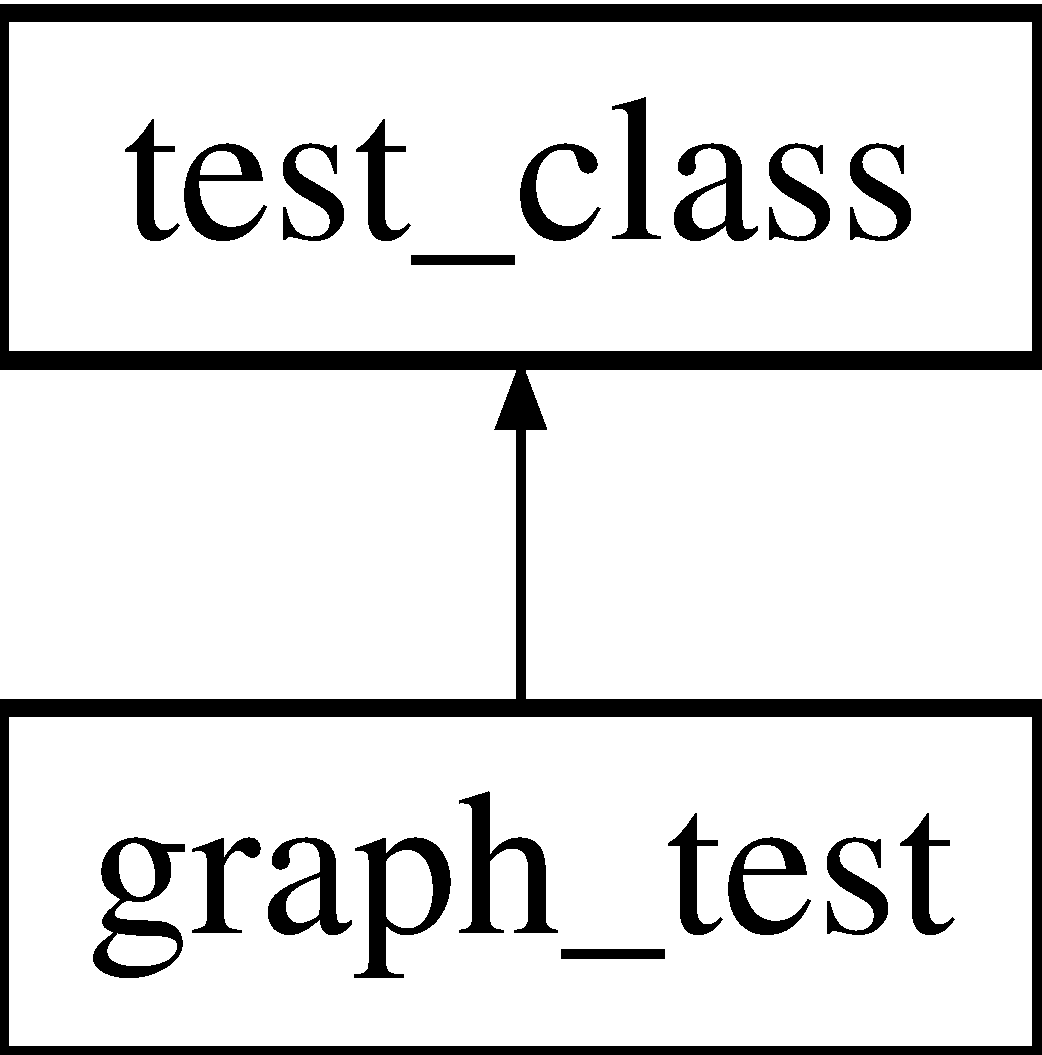
\includegraphics[height=2.000000cm]{classgraph__test}
\end{center}
\end{figure}
\subsection*{Protected Member Functions}
\begin{DoxyCompactItemize}
\item 
\hypertarget{classgraph__test_a5847cc3b842a645429000de955f17efc}{void \hyperlink{classgraph__test_a5847cc3b842a645429000de955f17efc}{test} ()}\label{classgraph__test_a5847cc3b842a645429000de955f17efc}

\begin{DoxyCompactList}\small\item\em Test data. \end{DoxyCompactList}\end{DoxyCompactItemize}
\subsection*{Additional Inherited Members}


\subsection{Detailed Description}
Testing of graph \begin{DoxyVerb}\end{DoxyVerb}
. 

The documentation for this class was generated from the following file\+:\begin{DoxyCompactItemize}
\item 
test\+\_\+graph.\+cpp\end{DoxyCompactItemize}

\hypertarget{classmystl_1_1graph_1_1MSTCompare}{\section{mystl\+:\+:graph$<$ Vertex\+Property, Edge\+Property $>$\+:\+:M\+S\+T\+Compare Class Reference}
\label{classmystl_1_1graph_1_1MSTCompare}\index{mystl\+::graph$<$ Vertex\+Property, Edge\+Property $>$\+::\+M\+S\+T\+Compare@{mystl\+::graph$<$ Vertex\+Property, Edge\+Property $>$\+::\+M\+S\+T\+Compare}}
}


Compare class used by M\+S\+T\+\_\+prim\+\_\+jarniks compares distance from cloud of two vertex iterators.  




{\ttfamily \#include $<$graph.\+h$>$}

\subsection*{Public Member Functions}
\begin{DoxyCompactItemize}
\item 
bool \hyperlink{classmystl_1_1graph_1_1MSTCompare_ac91ccaa0c8af200aa01fdc011eb644c2}{operator()} (const\+\_\+vertex\+\_\+iterator v, const\+\_\+vertex\+\_\+iterator u) const 
\begin{DoxyCompactList}\small\item\em compararator operator \end{DoxyCompactList}\end{DoxyCompactItemize}


\subsection{Detailed Description}
\subsubsection*{template$<$typename Vertex\+Property, typename Edge\+Property$>$class mystl\+::graph$<$ Vertex\+Property, Edge\+Property $>$\+::\+M\+S\+T\+Compare}

Compare class used by M\+S\+T\+\_\+prim\+\_\+jarniks compares distance from cloud of two vertex iterators. 

\subsection{Member Function Documentation}
\hypertarget{classmystl_1_1graph_1_1MSTCompare_ac91ccaa0c8af200aa01fdc011eb644c2}{\index{mystl\+::graph\+::\+M\+S\+T\+Compare@{mystl\+::graph\+::\+M\+S\+T\+Compare}!operator()@{operator()}}
\index{operator()@{operator()}!mystl\+::graph\+::\+M\+S\+T\+Compare@{mystl\+::graph\+::\+M\+S\+T\+Compare}}
\subsubsection[{operator()}]{\setlength{\rightskip}{0pt plus 5cm}template$<$typename Vertex\+Property, typename Edge\+Property$>$ bool {\bf mystl\+::graph}$<$ Vertex\+Property, Edge\+Property $>$\+::M\+S\+T\+Compare\+::operator() (
\begin{DoxyParamCaption}
\item[{const\+\_\+vertex\+\_\+iterator}]{v, }
\item[{const\+\_\+vertex\+\_\+iterator}]{u}
\end{DoxyParamCaption}
) const\hspace{0.3cm}{\ttfamily [inline]}}}\label{classmystl_1_1graph_1_1MSTCompare_ac91ccaa0c8af200aa01fdc011eb644c2}


compararator operator 


\begin{DoxyParams}{Parameters}
{\em v} & vertex iterator \\
\hline
{\em u} & vertex iterator \\
\hline
\end{DoxyParams}
\begin{DoxyReturn}{Returns}
if the distance of v is less than the distance of u 
\end{DoxyReturn}


The documentation for this class was generated from the following file\+:\begin{DoxyCompactItemize}
\item 
graph.\+h\end{DoxyCompactItemize}

\hypertarget{classmystl_1_1graph_1_1MSTLabel}{\section{mystl\+:\+:graph$<$ Vertex\+Property, Edge\+Property $>$\+:\+:M\+S\+T\+Label Class Reference}
\label{classmystl_1_1graph_1_1MSTLabel}\index{mystl\+::graph$<$ Vertex\+Property, Edge\+Property $>$\+::\+M\+S\+T\+Label@{mystl\+::graph$<$ Vertex\+Property, Edge\+Property $>$\+::\+M\+S\+T\+Label}}
}


Label class used by M\+S\+T\+\_\+prim\+\_\+jarniks stores a distance and vertex descriptor for the parent.  




{\ttfamily \#include $<$graph.\+h$>$}

\subsection*{Public Attributes}
\begin{DoxyCompactItemize}
\item 
\hypertarget{classmystl_1_1graph_1_1MSTLabel_a20782a95283cc0b02843d0e69a5c49b7}{double {\bfseries distance}}\label{classmystl_1_1graph_1_1MSTLabel_a20782a95283cc0b02843d0e69a5c49b7}

\item 
\hypertarget{classmystl_1_1graph_1_1MSTLabel_ab0a5bc456f2c64eeda2f2de8ac20b536}{size\+\_\+t {\bfseries parent}}\label{classmystl_1_1graph_1_1MSTLabel_ab0a5bc456f2c64eeda2f2de8ac20b536}

\end{DoxyCompactItemize}


\subsection{Detailed Description}
\subsubsection*{template$<$typename Vertex\+Property, typename Edge\+Property$>$class mystl\+::graph$<$ Vertex\+Property, Edge\+Property $>$\+::\+M\+S\+T\+Label}

Label class used by M\+S\+T\+\_\+prim\+\_\+jarniks stores a distance and vertex descriptor for the parent. 

The documentation for this class was generated from the following file\+:\begin{DoxyCompactItemize}
\item 
graph.\+h\end{DoxyCompactItemize}

\hypertarget{classtest__class}{\section{test\+\_\+class Class Reference}
\label{classtest__class}\index{test\+\_\+class@{test\+\_\+class}}
}


Test class for unit test framework \begin{DoxyVerb}\end{DoxyVerb}
.  




{\ttfamily \#include $<$unit\+\_\+test.\+h$>$}

Inheritance diagram for test\+\_\+class\+:\begin{figure}[H]
\begin{center}
\leavevmode
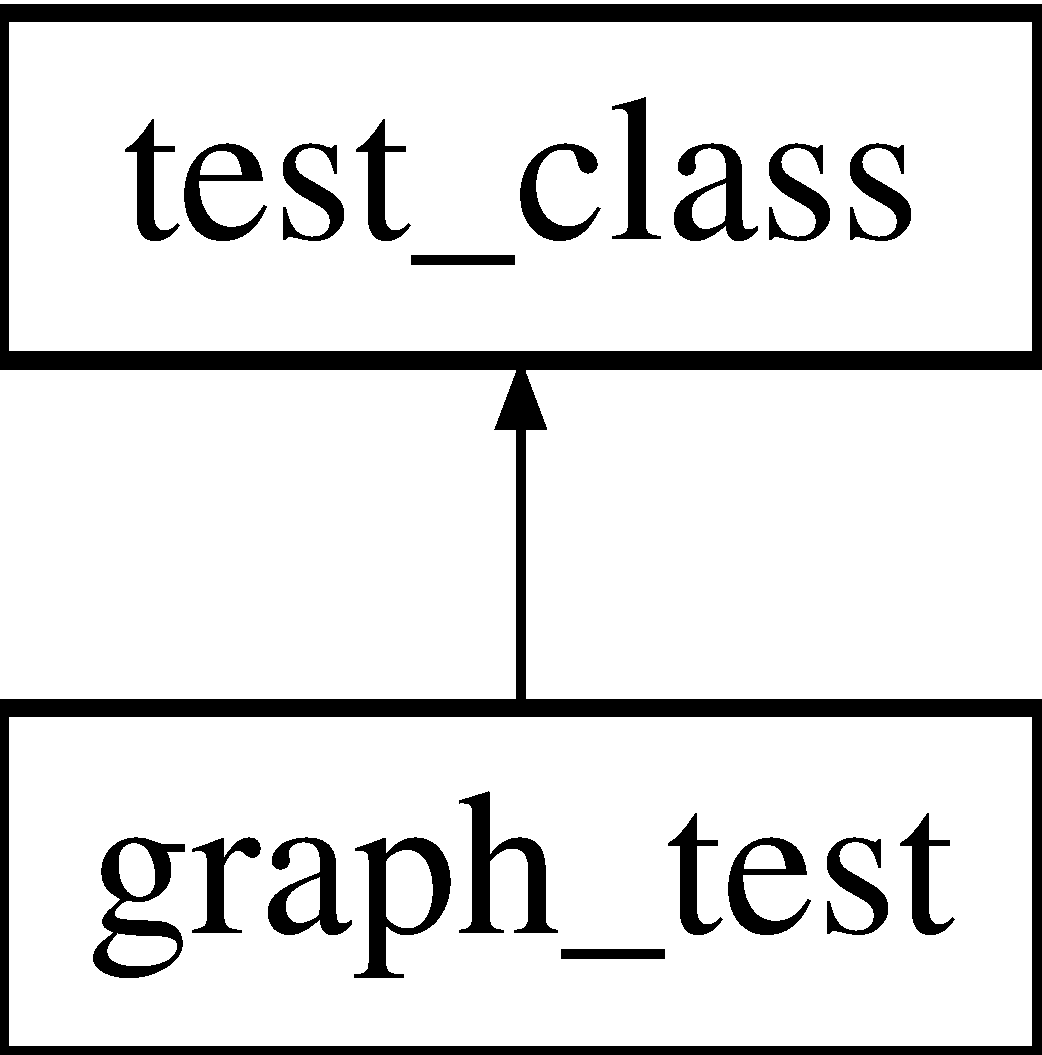
\includegraphics[height=2.000000cm]{classtest__class}
\end{center}
\end{figure}
\subsection*{Public Member Functions}
\begin{DoxyCompactItemize}
\item 
\hypertarget{classtest__class_aec748e707bc27bb28fe424722a975333}{\hyperlink{classtest__class_aec748e707bc27bb28fe424722a975333}{test\+\_\+class} ()}\label{classtest__class_aec748e707bc27bb28fe424722a975333}

\begin{DoxyCompactList}\small\item\em Constructor. \end{DoxyCompactList}\item 
\hypertarget{classtest__class_aadd18bb55da7e585c8628caa78b63c7b}{virtual \hyperlink{classtest__class_aadd18bb55da7e585c8628caa78b63c7b}{$\sim$test\+\_\+class} ()}\label{classtest__class_aadd18bb55da7e585c8628caa78b63c7b}

\begin{DoxyCompactList}\small\item\em Destructor. \end{DoxyCompactList}\item 
bool \hyperlink{classtest__class_a00fcb17fdfaf47816212afaeb108a743}{run} ()
\begin{DoxyCompactList}\small\item\em Run Unit test's setup, test, and teardown functions. \end{DoxyCompactList}\end{DoxyCompactItemize}
\subsection*{Protected Member Functions}
\begin{DoxyCompactItemize}
\item 
\hypertarget{classtest__class_a522c266a03c3aab7abc9b49e478e9154}{virtual void \hyperlink{classtest__class_a522c266a03c3aab7abc9b49e478e9154}{setup} ()}\label{classtest__class_a522c266a03c3aab7abc9b49e478e9154}

\begin{DoxyCompactList}\small\item\em Setup data to be tested. \end{DoxyCompactList}\item 
\hypertarget{classtest__class_ac0745ab8bcb4a3ff2d13b4c39c661215}{virtual void \hyperlink{classtest__class_ac0745ab8bcb4a3ff2d13b4c39c661215}{test} ()=0}\label{classtest__class_ac0745ab8bcb4a3ff2d13b4c39c661215}

\begin{DoxyCompactList}\small\item\em Test data. \end{DoxyCompactList}\item 
\hypertarget{classtest__class_a1231dba15477ba378c4a68995d3278cd}{virtual void \hyperlink{classtest__class_a1231dba15477ba378c4a68995d3278cd}{tear\+\_\+down} ()}\label{classtest__class_a1231dba15477ba378c4a68995d3278cd}

\begin{DoxyCompactList}\small\item\em Teardown data which was tested. \end{DoxyCompactList}\item 
bool \hyperlink{classtest__class_ac1111bb2bbb3a7870e5092cd5e6aee9b}{all\+\_\+tests\+\_\+passed} () const 
\item 
void \hyperlink{classtest__class_ac2a04ec6f3764fcfcd92fdefb205331a}{assert\+\_\+msg} (bool b, std\+::string msg)
\begin{DoxyCompactList}\small\item\em Assert a unit test passes. \end{DoxyCompactList}\end{DoxyCompactItemize}


\subsection{Detailed Description}
Test class for unit test framework \begin{DoxyVerb}\end{DoxyVerb}
. 

\subsection{Member Function Documentation}
\hypertarget{classtest__class_ac1111bb2bbb3a7870e5092cd5e6aee9b}{\index{test\+\_\+class@{test\+\_\+class}!all\+\_\+tests\+\_\+passed@{all\+\_\+tests\+\_\+passed}}
\index{all\+\_\+tests\+\_\+passed@{all\+\_\+tests\+\_\+passed}!test\+\_\+class@{test\+\_\+class}}
\subsubsection[{all\+\_\+tests\+\_\+passed}]{\setlength{\rightskip}{0pt plus 5cm}bool test\+\_\+class\+::all\+\_\+tests\+\_\+passed (
\begin{DoxyParamCaption}
{}
\end{DoxyParamCaption}
) const\hspace{0.3cm}{\ttfamily [inline]}, {\ttfamily [protected]}}}\label{classtest__class_ac1111bb2bbb3a7870e5092cd5e6aee9b}
\begin{DoxyReturn}{Returns}
All asserts have passed 
\end{DoxyReturn}
\hypertarget{classtest__class_ac2a04ec6f3764fcfcd92fdefb205331a}{\index{test\+\_\+class@{test\+\_\+class}!assert\+\_\+msg@{assert\+\_\+msg}}
\index{assert\+\_\+msg@{assert\+\_\+msg}!test\+\_\+class@{test\+\_\+class}}
\subsubsection[{assert\+\_\+msg}]{\setlength{\rightskip}{0pt plus 5cm}void test\+\_\+class\+::assert\+\_\+msg (
\begin{DoxyParamCaption}
\item[{bool}]{b, }
\item[{std\+::string}]{msg}
\end{DoxyParamCaption}
)\hspace{0.3cm}{\ttfamily [inline]}, {\ttfamily [protected]}}}\label{classtest__class_ac2a04ec6f3764fcfcd92fdefb205331a}


Assert a unit test passes. 


\begin{DoxyParams}{Parameters}
{\em b} & Conditional for assert \\
\hline
{\em msg} & Message on fail \\
\hline
\end{DoxyParams}
\hypertarget{classtest__class_a00fcb17fdfaf47816212afaeb108a743}{\index{test\+\_\+class@{test\+\_\+class}!run@{run}}
\index{run@{run}!test\+\_\+class@{test\+\_\+class}}
\subsubsection[{run}]{\setlength{\rightskip}{0pt plus 5cm}bool test\+\_\+class\+::run (
\begin{DoxyParamCaption}
{}
\end{DoxyParamCaption}
)\hspace{0.3cm}{\ttfamily [inline]}}}\label{classtest__class_a00fcb17fdfaf47816212afaeb108a743}


Run Unit test's setup, test, and teardown functions. 

\begin{DoxyReturn}{Returns}
Passed test or not 
\end{DoxyReturn}


The documentation for this class was generated from the following file\+:\begin{DoxyCompactItemize}
\item 
unit\+\_\+test.\+h\end{DoxyCompactItemize}

%--- End generated contents ---

% Index
\newpage
\phantomsection
\addcontentsline{toc}{chapter}{Index}
\printindex

\end{document}
